%
% 00_Einleitung.tex
%
% (c) 2020 Prof Dr Andreas Müller, Hochschule Rapperswil
%
% !TEX root = ../../buch.tex
% !TEX encoding = UTF-8
%
\section{Einleitung\label{jpeg:section:einleitung}}
\rhead{Einleitung}
\begin{figure}
    \centering
    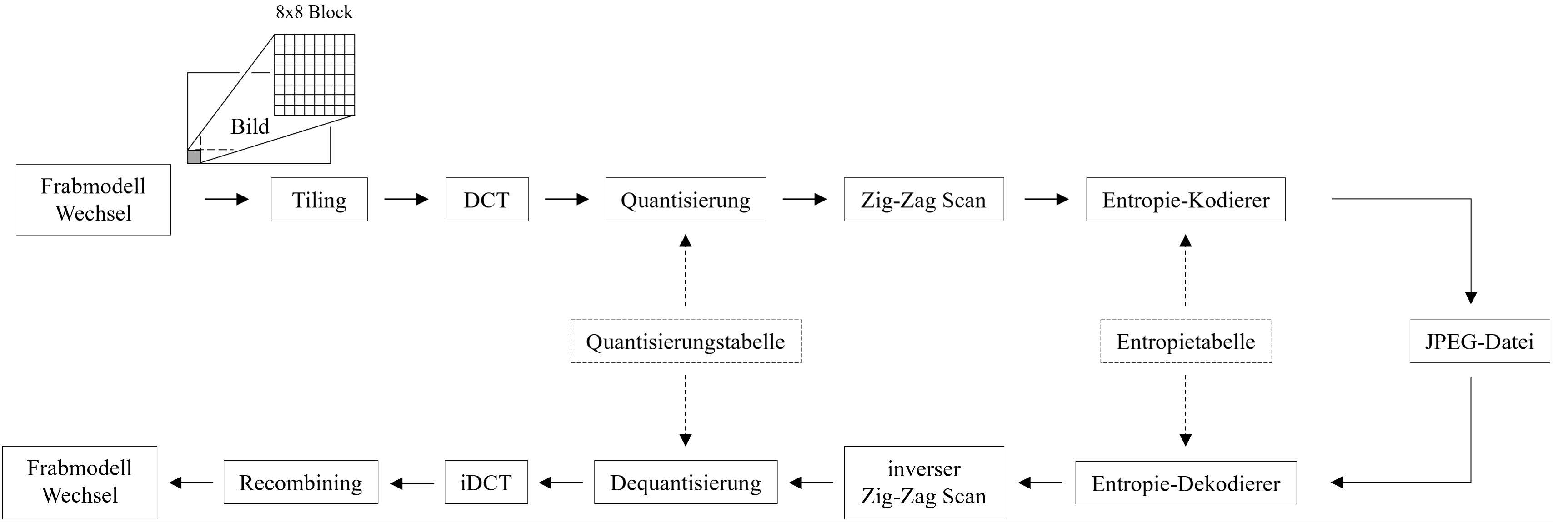
\includegraphics[width=\linewidth]{papers/jpeg/pictures/kompressionsschema.pdf}
    \caption{Vorgehen bei der Kompression und Dekompression von JPEG
        \label{jpeg:fig:kompressionsschema}}
\end{figure}
Sobald man Daten überträgt oder speichert, möchte man die effizienteste Form wählen, daher ist Datenkompression sehr naheliegend, das kann in vollständig rekonstruierbarer Form oder mit Verlusten erreicht werden.

Verlustloses Komprimieren gelingt, indem man einen Kodieralgorithmus auf die Daten anwendet und die redundanten Informationen wie in einem Wörterbuch speichert und jeweils darauf referenziert. Beim verlustbehafteten Verfahren werden die Daten, die für Menschen nicht erkennbar sind, entfernt um so den Inhalt zu reduzieren.

Es gibt inzwischen einige Methoden um Bilder zu komprimieren, in diesem Kapitel soll es um die beiden Algorithmen von der Joint Photographic Experts Group (JPEG) gehen.

Bilder werden zuerst mit einer Vorverarbeitung auf die Transformation vorbereitet, das sind Farb\-raum transformationen und Einteilung in kleinere Bereiche.
Anschliessend wird die Basistransformation durchgeführt und die Koeffizienten mit einer Tabelle quantisiert und ganzzahlig gerundet.
Die aus der Quantisierung entstandenen Werte werden Entropiekodiert, meisten wird das Prinzip von Huffman verwendet.
Die verwendete Methode wird im File abgelegt.
Zudem werden die Tabellen der unterschiedlichen Quantisierungen und Kodierungen mit abgespeichert, was in Abb. \ref{jpeg:fig:kompressionsschema} dargestellt wird.
Für die Dekompression werden diese Schritte rückwärts angewandt, wobei die verloren gegangenen Daten bei der Quantisierung nicht wieder hergestellt werden können. 

\subsection{Anwendung JPEG
\label{jpeg:subsection:anwendung}}
\rhead{Anwendung JPEG}
Grundlegend werden die Bilder mithilfe von verschiedenen Methoden in Basisfunktionen aufgeteilt, zu den jeweils die Koeffizienten berechnet werden, um diese in einem späteren schritt Manipulieren zu können und Daten einzusparen. 
Bei JPEG ist das die discrete cosine transform (DCT) und bei JPEG-2000 die discrete wavelet transform (DWT).
